\chapter{Architecture}

\section{Introduction}
\section{Prototype}
For demonstrating the architecture of this project we implement an architecture
prototype which shows basic functionality of sending a message from producer to 
consumer via broker. It fully implements the Kafka protocol for transmitting requests
and responses over network. Therefore the producer and consumer parts are compatible 
with Kafka itself. The broker part can handle any incoming request and either write or 
read from the file based log. 

The functionality of the architecture prototype can be split in two cases.
Case one covers producing a message and persisting in the brokers log:
\begin{figure}[H]
    \centering
    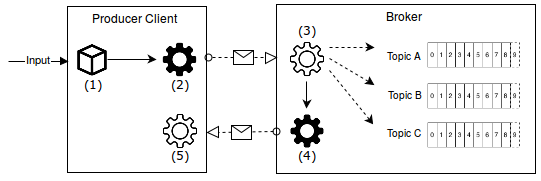
\includegraphics[width=0.9\textwidth]{images/concept_producer.png}
    \caption{Concept of Architecture Prototype Part I}
    \label{fig:conept-producer}
\end{figure}

\begin{table}[h]
\begin{tabular}{ll}
I   & Packing input message in data structure                                                          \\
II  & Serializing of data structure to byte string. The algorithm implements the Kafka protocol.       \\
III & Transmitting byte string via TCP socket over network                                             \\
IV  & Receiving and parsing byte string back to data structure                                         \\
V   & Write Message into topic specific log. The resulting file has same structure than the Kafka Log has.
\end{tabular}
\end{table}

Case two covers the part of consuming from a specific topic. Because Kafka works with 
pull-based consumption, the consumer fetch its messages with a constantly requesting it. 

\begin{figure}[H]
    \centering
   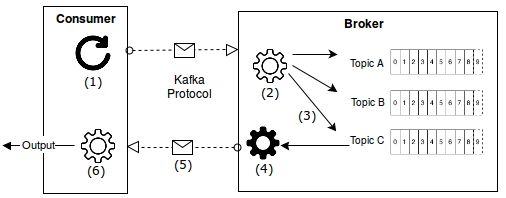
\includegraphics[width=0.85\textwidth]{images/concept_consumer.png}
    \caption{Concept of Architecture Prototype Part II}
    \label{fig:conept-consumer}
\end{figure}

\begin{table}[h]
\begin{tabular}{ll}
I   & Continuously send fetch request to broker implementing Kafka protocol \\
II  & Parse fetch request to data structure                                 \\
III & Read messages from log of specified topic                             \\
IV  & Serialize messages as response into byte string.                      \\
V   & Transmitting byte string back to consumer                             \\
VI  & Parse response from broker to get messages                           
\end{tabular}
\end{table}
